\section{The Ubhatob­yañ­janaka}
In the Theravāda Vinaya {\em Khandhaka} 1 we find the following passage:\footnote{Khandhaka 1 Pabbajjā PTS vol 1 page 89, translation by Ajahn Brahmali.}

\begin{quote}
{\em Tena kho pana samayena aññataro ubhatobyañjanako bhikkhūsu pabbajito hoti. So karotipi kārāpetipi. Bhagavato etamatthaṃ ārocesuṃ. Ubhatobyañjanako, bhikkhave, anupasampanno na upasampādetabbo, upasampanno nāsetabboti.}
\end{quote}

\begin{quote}
At one time an {\em ubhatob­yañ­janaka} had gone forth as a monk. He had sex and made others have it. They told the Buddha and he said, “An {\em ubhatob­yañ­janaka} should not be given the full ordination. If it has been given, he should be expelled.”
\end{quote}

Just like with the {\em paṇḍaka}, the {\em ubhatob­yañ­janaka} in this passage is already ordained at the time of this incident and in a similar way we can deduce that the rule itself is limited to {\em upasampadā} (full ordination) while novice ordination is allowed, while the commentarial texts mention that both are prohibited. And just like with the {\em paṇḍaka} we would expect the subject of the story to be expelled on the grounds of breaking the first rule against intercourse, but instead not only he but also all others like him are expelled. Again, there seems to be a prejudiced perception of these individuals as possessing an inherent flaw that makes them unable to keep their precepts.

For the term {\em ubhatob­yañ­janaka}\footnote{{\em Ubhato} meaning `in both ways, on both sides' and {\em byañjana} or {\em vyañjana} means `sign or mark'.} we have less material to go on than for the term {\em paṇḍaka}. They are only briefly mentioned in the Chinese Vinayas as those with two roots/faculties (二根) who are not allowed to ordain, but without any further explanation. The Therāvada Vinaya merely states that this person ``acted and was acted upon''. 

The commentarial literature is slightly more forthcoming but no less confusing as to the meaning of the word. The {\em Samantapāsādikā}\footnote{{\em Samantapādādikā}, vol. 3, para. 116. Translation by Ajahn Brahmali.} states:

\begin{quote}
{\em Ubhatobyañjanako bhikkhaveti itthinimittuppādanakammato ca purisanimittuppādanakammato ca ubhato byañjanamassa atthīti ubhatobyañjanako.Karotīti purisanimittena itthīsu methunavītikkamaṃ karoti. Kārāpetīti paraṃ samādapetvā attano itthinimitte kārāpeti, so duvidho hoti – itthiubhatobyañjanako, purisaubhatobyañjanakoti.Tattha itthiubhatobyañjanakassa itthinimittaṃ pākaṭaṃ hoti, purisanimittaṃ paṭicchannaṃ. Purisaubhatobyañjanakassa purisanimittaṃ pākaṭaṃ, itthinimittaṃ paṭicchannaṃ. Itthiubhatobyañjanakassa itthīsu purisattaṃ karontassa itthinimittaṃ paṭicchannaṃ hoti, purisanimittaṃ pākaṭaṃ hoti. Purisaubhatobyañjanakassa purisānaṃ itthibhāvaṃ upagacchantassa purisanimittaṃ paṭicchannaṃ hoti, itthinimittaṃ pākaṭaṃ hoti. Itthiubhatobyañjanako sayañca gabbhaṃ gaṇhāti, parañca gaṇhāpeti. Purisaubhatobyañjanako pana sayaṃ na gaṇhāti, paraṃ gaṇhāpetīti, idametesaṃ nānākaraṇaṃ.}
\end{quote}

\begin{quote}
The {\em ubhatob­yañ­janaka} means: Because of kamma giving rise to female characteristics and kamma giving rise to male characteristics, there is for them the characteristics of both. With the male characteristic they act to transgress through sexual intercourse with women. Having encouraged another, they cause action in their own female characteristic. 

They are twofold: the female {\em ubhatob­yañ­janaka} and the male {\em ubhatob­yañ­janaka}. In regard to this, the female characteristic of the female {\em ubhatob­yañ­janaka} is apparent, but the male characteristic is hidden. The male characteristic of the male {\em ubhatob­yañ­janaka} is apparent, but the female characteristic is hidden. 

While the female {\em ubhatob­yañ­janaka} is acting with manliness among women, the female characteristic is hidden, whereas the male characteristic is apparent. 
When the male {\em ubhatob­yañ­janaka} enters the state of a woman for the sake of men, the male characteristic is hidden, whereas the female characteristic is apparent. 
The female {\em ubhatob­yañ­janaka} becomes pregnant and causes others to become pregnant. The male {\em ubhatob­yañ­janaka} does not become pregnant, but causes others to become pregnant. This is the difference between them.
\end{quote}

The sub-commentary\footnote{Vmv.3.116, translation by Ajahn Brahmali.} adds the following: 
\begin{quote}
{\em Ubhinnampi cesaṃ ubhatobyañjanakānaṃ yadā itthiyā rāgo uppajjati, tadā purisabyañjanaṃ pākaṭaṃ hoti, itaraṃ paṭicchannaṃ. Yadā purise rāgo uppajjati, tadā itthibyañjanaṃ pākaṭaṃ hoti, itaraṃ paṭicchannaṃ.}
\end{quote}

\begin{quote}
For both {\em ubhatob­yañ­janakas}, when lust for a woman arises, then the male characteristic is apparent, whereas the other is hidden, and when lust for a man arises, then the female characteristic is apparent, whereas the other is hidden.
\end{quote}

The Chinese equivalent of the Pali {\em Samantapāsādikā} can be found in T24 1462: 善見律毘婆沙:\footnote{T24 1462 善見律毘婆沙 0792c03–0792c06. 5\textsuperscript{th} Century CE.}
\begin{quote}
There are three kinds of two-facultied people (二根): those who can impregnate and conceive. Those who can impregnate but not conceive, and those who cannot impregnate but who can conceive. These three types of people are not allowed to become monks and take the full precepts. If they have already taken the full precepts, they should be expelled.
\end{quote}

Other Chinese commentaries have variations of the same passage:\footnote{See f.i. Shinsan X44 0744 四分律名義標釋 0450b01–0450b04.}
\begin{quote}
It is said that a person has two roots/faculties (二根): male and female. There are three kinds: The first is able to self-reproduce. He can impregnate and conceive. The second can impregnate others but cannot conceive himself. The third type cannot impregnate but he can conceive when impregnated by another. 
\end{quote}

The {\em Samantapāsādikā} identifies two types of {\em ubhatob­yañ­janakas} while the Chinese commentaries identify three. The {\em Samantapāsādikā}'s explanation is all the more puzzling because it describes the female {\em ubhatob­yañ­janaka} as having apparent female characteristics and the male characteristics hidden, but if they feel attracted to a women, they seem to be able to hide the female characteristic and make the male characteristic apparent. The opposite is described for a male {\em ubhatob­yañ­janaka}. Moreover the female {\em ubhatob­yañ­janaka} is able to become pregnant but also impregnate others so they become pregnant. This last aspect is also mentioned as one of the three types in the Chinese commentaries. The other two types in the Chinese are just described as being able to either get pregnant or impregnate others, just like females and males but with no further explanation as to why they are different from females and males. 

Apparently the ability to procreate is very important here and I would like to point out that it is humanly impossible to both conceive and impregnate.\footnote{In Appendix \ref{appendix3}, section \ref{hermaphrodite} I have described our current medical understanding of what it entails to both procreate as a male and a female.} However, as we have seen in the Vedic mythology this is a recurrent theme and there are many instances where a person is both mother and father. King Ila himself, in the form of the woman Ilā, becomes pregnant and bears a son. He/she is bound to keep on changing sex/gender which also results in a change in sexual desires. In the {\em Mahābārata Anuśāsanaparvan}\footnote{MBh 13.12.} we find the tale of King Bhaṅgāśvana, who is longing for a son, and performs a divine ritual as a result of which he gets one hundred sons, but in doing so invokes the anger of the god Indra, who turns him into a woman. As a woman she conceives another hundred sons. 

Also in the Buddhist scriptures, in the story of Sorreya\footnote{See \cite{dhammadinna} for a detailed analysis of this story that appears in the {\em Soreyyatthera-vatthu} of the {\em Dhammapada-aṭṭhavaṇṇanā}. The {\em Dhammapada-aṭṭhavaṇṇanā} was seemingly translated from Pali into Sinhalese by Buddhaghosa on the invitation of an otherwise unknown Kumārakassapa Thera. Buddhaghosa is mentioned as the author in the epilogue of this work at Dhp-a IV 235–236.}, we find a similar account whereby somebody changes sex and gender involuntarily due to their `instant kamma’, triggered by impure thoughts. The difference with the Vedic stories is that the sex-change is attributed to causality and not to a spell or curse. This shows an underlying assumption of gender inequality, namely that the male sex is preferred and the result of `good kamma', while the female sex is a result of `bad kamma'.

\bigskip
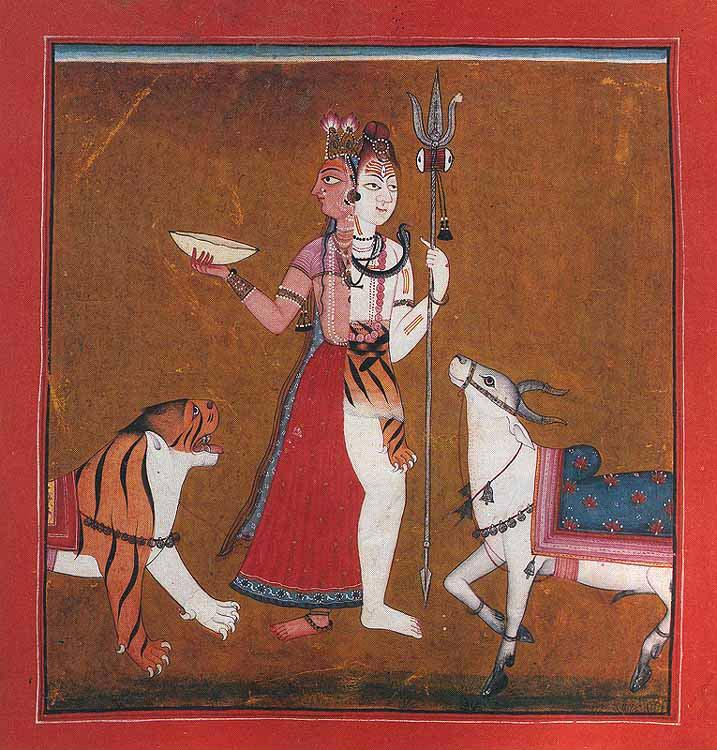
\includegraphics[width=\textwidth]{androgyne.jpg}
\begin{minipage}{\textwidth}
\captionof{figure}{Śiva in their androgynous form of Ardhanārīśwara}
\end{minipage}
\label{siva}

There are also many instances in the Vedic mythology where a sex/gender change is a deliberate choice. Gods are able to enact a sex/gender change in others, but also use it themselves for a variety of reasons, most notably for the purpose of sexual intercourse. One well-known story is the story of Kṛṣṇa who transforms himself into a woman in order to marry and have sex with Aravan. This story is reenacted each year by men who dress as women or who are {\em hijras} during the {\em thali} festival\footnote{See \cite{goldman} page 388 and \cite{nanda} page 21.}. Another story is recounted in the {\em Mahā Bhāgavata Purāṇa} where the gods Śiva and Kāli both change gender in order to experience sexuality from the perspective of the other\footnote{See \cite{wendy} page 334.}. Another reason for a deliberate sex change is to destroy the power of meditative yogis. Celibate men (and therefore celibate monks) are seen as particularly powerful and can only be defeated if a god changes himself into a female form to seduce them or gets a woman to do so for him\footnote{See \cite{wendy1969} for detailed stories whereby yogis were seduced to break their power.}. The gods Visnu and Śiva (see Figure 2) change sex/gender frequently\footnote{Wendy \cite{wendy} gives a particularly interesting account on androgyns in the ancient texts. These androgyns can have a large variety of possible characteristics and origins. See for instance pages 261–313 for detailed stories.}.

According to Serena Nanda\footnote{Serena \cite{nanda} quotes Bullough pages 21–22.}, Tantric Hinduism holds that all persons contain both male and female principles within themselves. The Supreme Being is conceptualized as a complete hermaphrodite, which is the ideal. In some sects, males (never females) imitate women in dress and behavior to achieve salvation or to realize the woman in themselves in order to reach true love.

The other types of {\em ubhatob­yañ­janakas} mentioned in the commentaries seem to be similar in their ability to have sex as both a male and a female, but being sterile in one of these faculties. Again, this is not something we naturally find in human beings but it is a theme extensively found in the Vedic myths.

% A story of a slightly different genre is recounted in the Buddhist {\em Dīrghāgama} Sutra T24 which describes how in the beginning all beings were male or female and were therefore subject to marriage. But the heavenly beings were bestowed with the gift of being free from marriage with no distinction between male and female and all became hermaphrodites (二根) with exactly the same faculties. This passage seems slightly different from the above because here the shift is not from male to female or visa versa but to a hermaphrodite and only bestowed on heavenly beings. So the same word 二根 is used for a hermaphrodite here but it is also seen as a great gift.

The word {\em ubhatob­yañ­janaka} does not appear in any texts outside of the Buddhist Vinaya and the Vinaya commentaries.\footnote{Appendix \ref{appendix2}, Figure 4 shows that the word {\em ubhatob­yañ­janaka} does not appear in any Vedic or Brahmanical texts and only appears in the Buddhist texts. There is however another word in the {\em Varṣāvastu}, namely {\em strīpuruṣapaṇḍakam} which literally means a {\em paṇḍaka} who is both female and male.} It seems however logical that by the sheer definition of the {\em napuṃsaka} as `anything that is not entirely male or female' the term {\em ubhatob­yañ­janaka} also falls under this category. As a sub-category of the {\em napuṃsaka} they would have been seen as hyperlibidinous, which is explained in later texts by the fact that {\em napuṃsakas} have both male and female characteristics.\footnote{As we have seen in chapter \ref{linga} it is likely that `characteristics' are defined as more than merely genital or procreative. \cite{jackson}, quoting Bunmi Methangkun (1986) (article in Thai), observes that psychological as well as physiological factors are involved in the constitution of the {\em ubhatob­yañ­janaka}. He also observes (without reference) that in early Buddhist communities men who engage in receptive anal sex are seen as feminized and thought to be hermaphrodites.}. The explanation in the commentaries and sub-commentary as mentioned above also shows they are seen as bisexual in nature, similar to what we have seen in the Jain commentarial literature description of {\em napuṃsaka}.

The term {\em paṇḍaka} as a subset of {\em napuṃsaka} was also seen as having both male and female characteristics in the Jain scriptures but is obviously not the same as the {\em ubhatob­yañ­janaka}. The difference between the {\em paṇḍaka} and the {\em ubhatob­yañ­janaka} clearly seems to be on the procreative level in that the {\em ubhatob­yañ­janaka} is able to conceive and impregnate while the {\em paṇḍaka}, as an impotent man, can do neither. From the descriptions given in the {\em Samantapāsādikā} we can also conclude that the {\em ubhatob­yañ­janaka} is able to change their primary and secondary characteristics, including outside appearance and behavior to appear either male or female. Again, this is not possible outside the realm of mythology.

All the Vinayas agree that the {\em ubhatob­yañ­janaka}/二根 is one of the four sex/gender types next to male, female and {\em paṇḍaka}/黃門. Considering that the male and female were seen as both having just one root/faculty (in the meaning of procreative ability), and the {\em paṇḍaka} has none\footnote{Note that when the {\em paṇḍaka} appears in the texts in the list of these four sex/gender types, it is always described in the Chinese Vinayas with the characters 黃門 (`eunuch') and never as 不能男 (`impotent'). Indeed we find in the Chinese texts that a eunuch is somebody with the `male faculty' removed. There might be some confusion here as to what entails characteristics and the Chinese scribes would have only been able to describe this based on their own experiences in their own culture.}, the person with two faculties fills a gap. Bee Scherer notes that this fourfold taxonomy (`male', `female', `both ...', `neither ...') is intended to achieve the Classical Indian (and especially Buddhist) fourfold logical tetralemma called the {\em catuṣkoṭi}\footnote{See \cite{scherer} page 68 and Dr. M. Vermeulen, whose book on this subject is yet to be published.} and that the categories of {\em paṇḍaka} and {\em ubhatob­yañ­janaka} are largely academic. This might indeed have played a role but I believe there are also other considerations like the fact that these types, either as mythological beings or the reenactment thereof, are indeed found in India.

Just like the term {\em paṇḍaka}, I believe that the {\em ubhatob­yañ­janaka} is a later addition to the Vinaya. The word does not appear in the early Suttas nor in the {\em Pāṭimokkha} or other early parts of the Vinaya\footnote{See Appendix \ref{appendix2}, Figure 3.} and only briefly in the Vinaya. The description is so brief and hardly existent in the Chinese texts that it seems to be added almost as an after-thought. The insertion would have most likely occurred during the redaction of the Vinaya at the Second Council as discussed in the previous chapter.

The {\em ubhatob­yañ­janaka} seems to be a rather elusive term that does not allow itself to be captured easily. Various scholars have tried to explain this as a form of intersex\footnote{For a brief description of the term `intersex' see Appendix \ref{appendix3}, section \ref{intersex}.} for the sole reason that intersex people were previously erroneously called `hermaphrodite' and a hermaphrodite can procreate in both the male and female way as in the description of the {\em ubhatob­yañ­janaka} in the commentaries. This is confusing as a true hermaphrodite does not exist among humans and is distinct from intersex. 

From the descriptions in the commentaries, the {\em ubhatob­yañ­janaka} is not human in nature. It is a concept, a mythological being, the embodiment of the feminine principle in the male. And just like the {\em paṇḍaka} it is likely that there were also people involved in the religious enactment of these mythological tales as we have seen in Tantric Hinduism, which would have included strong sexual motifs\footnote{See \cite{nanda} page 22.}. It is likely that people with ambigious genital characteristics were among these, as they naturally bear some resemblance to the idealized hermaphrodite Supreme Being, but the concept was more than just entailing physical characteristics; it also involved gender-expression and social religious roles. As Robert \cite{goldman} points out: ``... the whole phenomenon appears to be deeply bound up with a patriarchal culture's ambivalent construction of women and their sexuality.'' The Vedic stories explore the deep longing of men to be able to conceive and this idea is found in a variety of Indian sources. Again, this is a concept that does not match any contemporary notions.
